\documentclass[sigplan,screen]{acmart}\settopmatter{printfolios=true,printccs=false,printacmref=false}
%\documentclass[acmsmall,review,anonymous]{acmart}\settopmatter{printfolios=true,printccs=false,printacmref=false}

\usepackage[utf8]{inputenc}
\usepackage[T1]{fontenc}

\usepackage{adjustbox}
\usepackage{booktabs}
\usepackage{listings}
\usepackage{multicol}
\usepackage[autolanguage]{numprint}
\usepackage{proof}
\usepackage{softdev}
\usepackage{subcaption}
\usepackage{wrapfig}
\usepackage{xspace}
\usepackage{menukeys}

\usepackage[ruled]{algorithm2e} % For algorithms
\renewcommand{\algorithmcfname}{ALGORITHM}
\SetAlFnt{\small}
\SetAlCapFnt{\small}
\SetAlCapNameFnt{\small}
\SetAlCapHSkip{0pt}
\IncMargin{-\parindent}

\acmJournal{PACMPL}
\acmVolume{1}
\acmNumber{CONF} % CONF = POPL or ICFP or OOPSLA
\acmArticle{1}
\acmYear{2018}
\acmMonth{1}
\acmDOI{} % \acmDOI{10.1145/nnnnnnn.nnnnnnn}
\startPage{1}

\lstset{
    basicstyle=\ttfamily\scriptsize,
    xleftmargin=0pt,
    numbersep=.8em,
    numberstyle=\scriptsize\tt\color{gray},
    captionpos=b,
    escapeinside={{<!}{!>}},
}

% from https://tex.stackexchange.com/questions/264361/skipping-line-numbers-in-lstlisting#264373
\let\origthelstnumber\thelstnumber
\makeatletter
\newcommand*\Suppressnumber{%
  \lst@AddToHook{OnNewLine}{%
    \let\thelstnumber\relax%
     \advance\c@lstnumber-\@ne\relax%
    }%
}

\newcommand*\Reactivatenumber[1]{%
  \setcounter{lstnumber}{\numexpr#1-1\relax}
  \lst@AddToHook{OnNewLine}{%
   \let\thelstnumber\origthelstnumber%
   \refstepcounter{lstnumber}
  }%
}

\setcopyright{none}

\bibliographystyle{ACM-Reference-Format}
\citestyle{acmauthoryear}

% DOI
%\acmDOI{0000001.0000001}

% Paper history
%\received{February 2007}

\newcommand{\inputtree}[0]{\emph{CST}\xspace}
\newcommand{\eco}[0]{\emph{Eco}\xspace}
\newcommand{\ald}[0]{\emph{ALD}\xspace}
\newcommand{\qtt}[1]{`\texttt{#1}'\xspace}

\newcommand{\hotkeynewlbox}[0]{\keys{Ctrl+L}\xspace}
\newcommand{\hotkeyleavelbox}[0]{\keys{Ctrl+Shift+L}\xspace}

\lstnewenvironment{lstdefault}[1][]
  {
    \lstset{
        numbers=left,
        language=Python,
        keywordstyle=\color{red!70!black},
        commentstyle=\itshape\color{gray!90!black},
        stringstyle=\color{green!60!black},
        basicstyle=\linespread{1.0}\footnotesize\ttfamily,
        numberstyle=\tiny,
        keepspaces=true,
        breaklines=true,
        captionpos=b,
        abovecaptionskip=0.8em,
        columns=fullflexible,
        xleftmargin=10pt,
        aboveskip=1em,
        belowskip=0em,
        showstringspaces=false,
        literate={\$}{{\$}}1,
        escapeinside={{<!}{!>}},
        #1
    }
}{}

\lstdefinelanguage{EcoGrammar}
{
    alsoletter={:,\:=,|},
    morekeywords={:, =, | },
    keywordstyle=\color{red!70!black},
    morestring=[b]",
    stringstyle=\color{green!60!black},
    commentstyle=\itshape\color{gray!90!black},
    comment=[l]{//},
    morecomment=[s]{/*}{*/},
}

\lstnewenvironment{lsteco}[1][]
  {
    \lstset{
        language=EcoGrammar,
        basicstyle=\footnotesize\ttfamily,
        numberstyle=\tiny,
        xleftmargin=10pt,
        showstringspaces=false,
        #1
    }
}{}

% Document starts
\begin{document}
% Title portion. Note the short title for running heads
\title{Automatic Language boxes}

\author{Lukas Diekmann}
\affiliation{%
  \department{Software Development Team}
  \institution{King's College London}
  \country{United Kingdom}}
\author{Laurence Tratt}
\orcid{0000-0002-5258-3805}
\affiliation{%
  \department{Software Development Team}
  \institution{King's College London}
  \country{United Kingdom}
}
\thanks{Authors' URLs: %
    L.~Diekmann~\url{http://lukasdiekmann.com/},
    L.~Tratt~\url{http://tratt.net/laurie/}.
}


\begin{abstract}
\end{abstract}

\keywords{Parsing, language composition, programming languages}

\maketitle

\section{Introduction}

Incremental parsers are based on traditional parsing algorithms. However,
instead of parsing a whole file each time the program is executed, incremental
parsers generate and update a parse tree from the user input as the user types.
When editing a program, this parse tree is then modified directly,
e.g.~changing the name of a variable directly updates the value of the token in
the parse tree that represents that variable. After each edit the incremental
parser updates and reparses the relevant parts of the parse tree, attempting to
reuse as many unchanged parts of the tree as possible. This is not only faster
than parsing the entire program from scratch, but also has the added benefit
that meta-data on parse tree nodes is kept intact when the program is reparsed.

Editing programs this way allows us to embed languages into one another without
separators, by using language boxes. These boxes can be manually inserted by
the user to write code in another language. When creating a new language box,
it is inserted directly into the parse tree. Each language box has its own
parse tree which is maintained by its own incremental parser. This way
languages stay completely separated from each other which bypasses all
ambiguity problems. For example, when editing a program in language \emph{X},
the user can at any point insert a language box for language \emph{Y}. Typing
inside of that box edits in language \emph{Y}, while typing outside of the box
edits in language \emph{X}. Programs may contain any number of languages
boxes, and language boxes can be nested arbitrarily deep.

The main problem with language boxes is that they need to be inserted manually
by the user, which in some cases can seem tedious and unnecessary. In this
paper we propose a solution on how how language boxes can be inserted
automatically and without the need for user interaction in many useful
scenarios. This paper introduces a new algorithm that allows an editor to
detect when a user writes code that is intended for a language box. It can then
create that box automatically and wrap the written code in it. The goal is to
improve the user's workflow, which previously required them to insert language
boxes explicitly and manually.  Since many language compositions are ambiguous
it is impossible to perfectly predict the user's intentions. Fortunately, it is
possible to do a decent enough job by employing heuristics, which can be
improved further by manually tweaking compositions to deal with some language
specific edge cases.

The paper is structured as follows: Section \ref{sec_background} gives an
overview on incremental lexing and parsing which is the basis for language
composition via language boxes. Section \ref{sec_finding_lbox_candidates}
describes how we can use parsing errors to find automatic language boxes, how
we can present multiple solutions to the user, and how automatically inserted
language boxes can also automatically be removed again. Section
\ref{sec_lbox_limitations} describes some of the limitations of automatic
language boxes, e.g.~where either unwanted language boxes are inserted or
detection fails and no language box is inserted at all. Section
\ref{sec:impl_defaultrec} describes the implementation of recognisers, which
are used during the detection of automatic language boxes.

\section{Background}
\label{sec_background}

Traditional parsing is a batch process: an entire file is fed through a parser
and a parse tree is created from it. Incremental parsing, in contrast, is an
online (i.e.~interactive) process: it parses text as the user types and
continually updates a parse tree.  In other words, incremental parsing allows
an editor to reparse a program after every keypress, resulting in an always
up-to-date parse tree, which can then be used for semantic analysis or syntax
highlighting.  A number of incremental parsing algorithms were published from
the late 70s~\cite{ghezzi79incremental, jalili82building, larcheveque95optimal,
petrone95reusing} to the late 90s, gradually improving efficiency and
flexibility~\cite{li97new,ferro94efficient}.  The last major work in this area
was done in 1998 by \cite{wagner98practicalalgorithms} who defined a number of
incremental parsing algorithms. His LR-based incremental parser has two major
benefits: it handles the full class of $\textrm{LR}(k)$ grammars; and has
formal guarantees that the algorithm is optimal (i.e.~the number of steps
needed to integrate user changes into an existing parse tree is minimal).
Furthermore, Wagner presents an algorithm for incremental lexical analysis,
improving on works such as \cite{fischer84poe, bahlke86psg, ballance92pan,
fischer92aladin}. The following gives a brief overview of incremental lexing
and parsing.

An incremental parser and lexer both operate on a parse tree. Parse tree nodes
are either \emph{nonterminals} (representing rules in the grammar) or
\emph{tokens} (representing terminal symbols). Nonterminal nodes are immutable
(i.e.~their type cannot change) and have zero or more ordered child nodes
(which are not immutable and can be updated). Tokens have a type (e.g.~`int')
and a value (e.g.~`3') and are mutable. Figure \ref{fig_example_parsetree}
shows an example of a parse tree.

\begin{figure}
\begin{minipage}[b]{0.17\textwidth}
\begin{lsteco}
// Parser
Var: Id "eq" Val;
Id: "id";
Val: "int";

// Lexer
eq:"="
id:"[a-z]+"
int:"[0-9]+"
\end{lsteco}
\end{minipage}
\begin{minipage}[b]{0.30\textwidth}
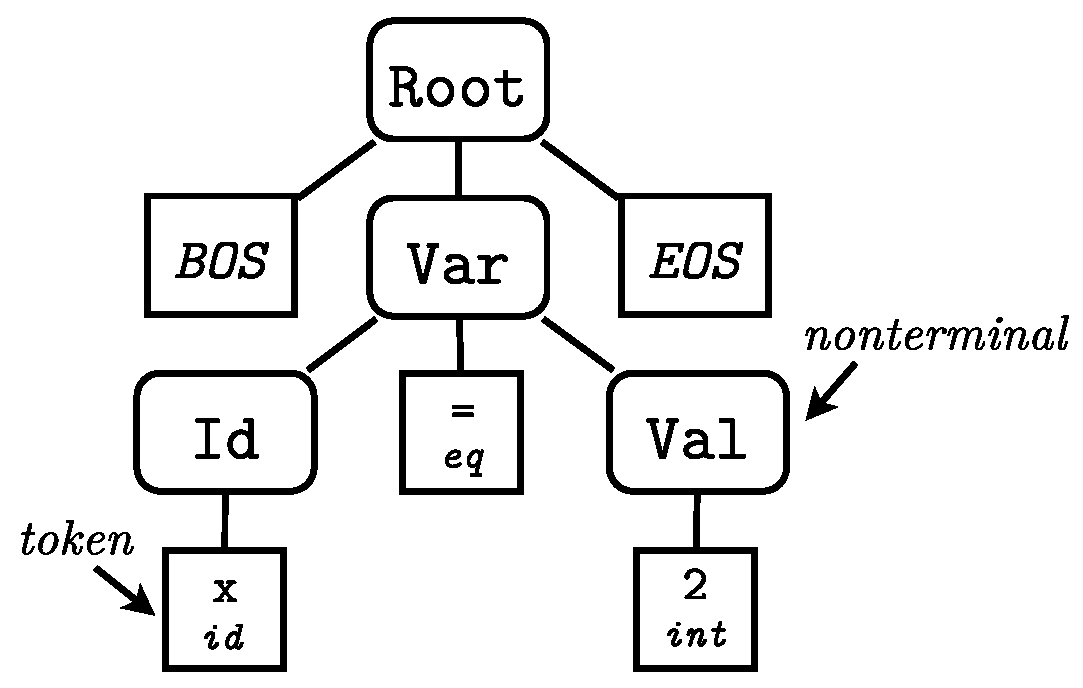
\includegraphics[width=1.0\textwidth]{images/sampleparsetree}
\end{minipage}
\caption{An example of a parse tree constructed from the grammar on the left.
The minimal parse tree consists of three
special nodes: a \emph{Root} nonterminal; and \emph{BOS} (Beginning of
Stream) and \emph{EOS} (End of Stream) terminals (both children of
\emph{Root}). For brevity reasons, these nodes are elided for the remainder of
this thesis. All nodes created from user input are (directly or indirectly)
children of \emph{Root} and are contained between \emph{BOS} and \emph{EOS}.}
\label{fig_example_parsetree}
\end{figure}

When the user types, the incremental lexer first either creates, or updates,
tokens in the parse tree. The lexer considers where the cursor is in the tree
(i.e.~where the user is typing) and uses lookahead knowledge stored in the
tokens to work out the affected area of the change. Newly created tokens are
then merged back into the tree.  In the simple case where a token's value, but
not its type, was changed, no further action is needed. In all other cases, the
path from each changed token up to the root is first marked with \textit{nested
change} flags which are then used by the incremental parser to update the parse
tree. The incremental parser starts at the beginning of the tree and tries to
reparse all subtrees that contain changes. Assuming the user's input is
syntactically valid, nonterminals are created or removed, as appropriate.
Unchanged subtrees are reused as is whenever possible. Since nonterminals are
immutable, subtrees which can't be reused must be recreated from scratch.

Syntactically incomplete programs lead to temporarily incorrect parse trees.
In such cases, the incremental parser typically attaches tokens to a single
parent. When the user eventually creates a syntactically valid program, the
tree is rewritten.

\subsection{Language boxes}

Language boxes allow users to embed one language inside another.  Language
boxes have a type (e.g.~HTML), an associated editor (e.g.~an extended
incremental parser), and a value (e.g.~a parse tree).  By design, language
boxes only consider their own contents ignoring parent and sibling language
boxes. It is therefore necessary to define the notion of the CST (Concrete
Syntax Tree), which is a language box agnostic way of viewing the user's input.
Different language box editors may have different internal tree formats, but
each exposes a consistent interface to the CST.  Put another way, the CST is a
global tree which integrates together the internal trees of individual language
boxes.

Language boxes fit naturally with the incremental parser due to a property of
CFGs which is rarely of consequence to batch-orientated parsers: parsers only
need to know the type of a token and not its value. In this incremental parser
approach, nested language boxes are therefore treated as tokens. When the user
inserts an SQL language box into Python code, a new node of type \texttt{SQL}
is inserted into the parse tree and treated as any other token. From the
perspective of the incremental parser for the Python code, the language box's
value is irrelevant as is the fact that the language box's value is mutable.
Language boxes can appear in any part of the text, though, in this example, an
SQL language box is only syntactically valid in places where the Python grammar
makes a reference to the SQL grammar. Nested language boxes which use the
incremental parser have their own complete parse trees, as can be seen in
Figure~\ref{fig:lboxtree}.

\begin{figure}[t]
\begin{center}
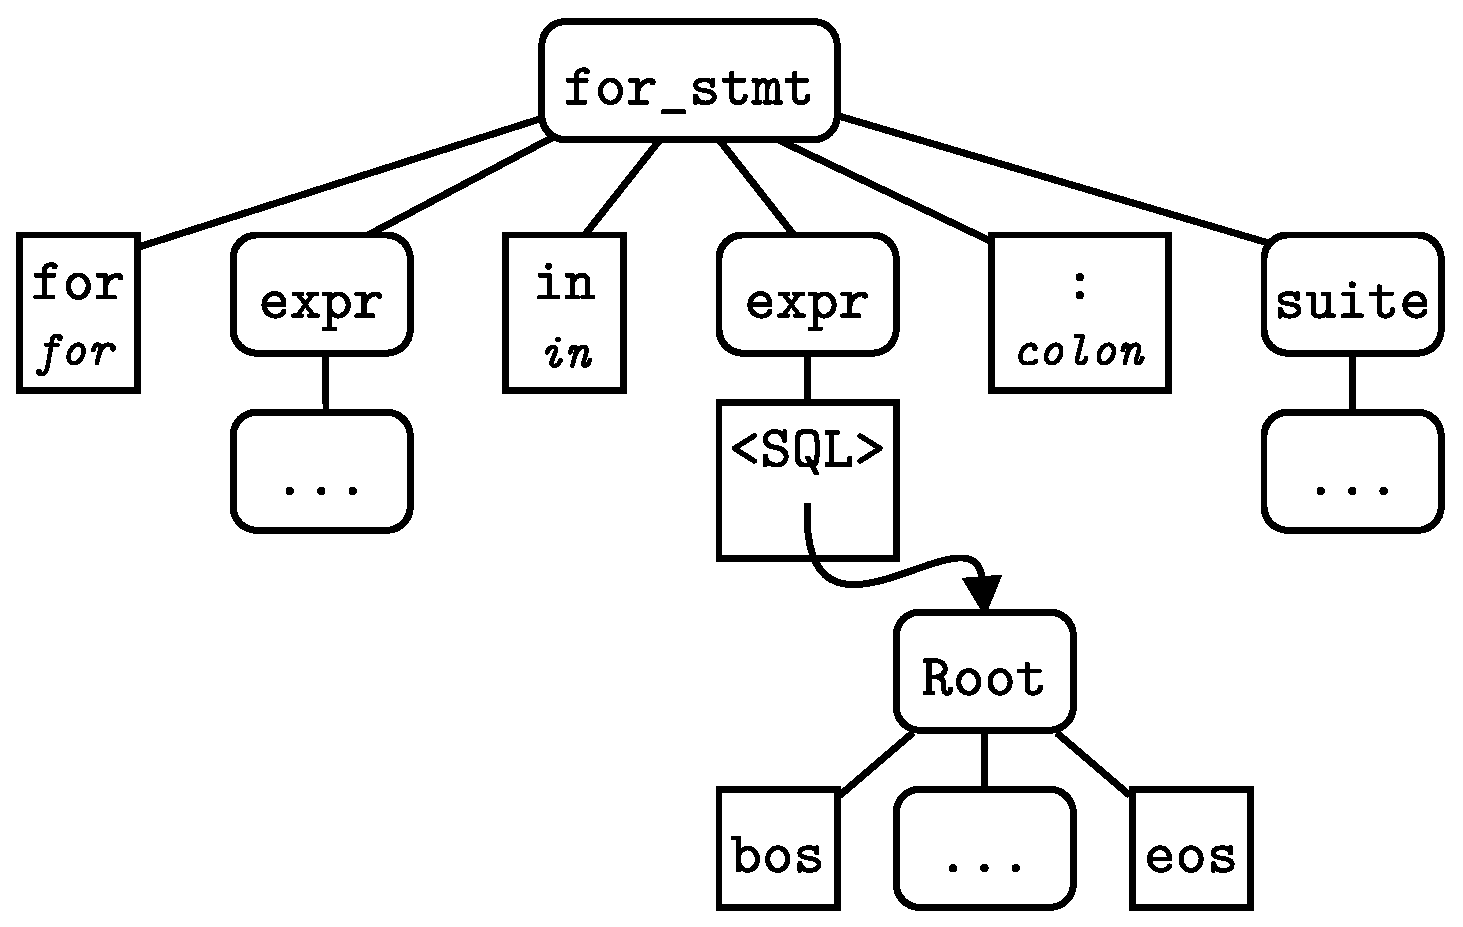
\includegraphics[width=0.35\textwidth]{images/lboxtree}
\caption{An elided example of an SQL language box nested within an outer Python
language box. From the perspective of the incremental parser, the tree stops
at the SQL token. However, we can
clearly see in the above figure that the SQL language box has its own parse
tree, which thus forms part of the wider \inputtree.}
\label{fig:lboxtree}
\end{center}
\end{figure}

When an end-user creates a new file in \eco, they are asked to specify
which language that file will be written in. Let us assume that they choose the
composed language named (unimaginatively) HTML+Python+SQL which composes
the modular HTML, Python, and SQL languages within \eco. Although
users can write whatever code they want in \eco, this composed language
has the following syntactic constraints: the outer language must
be HTML; in the outer HTML language, Python language boxes can be inserted
wherever HTML elements are valid (i.e.~not inside HTML tags); SQL language boxes
can be inserted anywhere a Python statement is valid; and HTML language boxes
can be inserted anywhere a Python statement is valid (but one cannot nest
Python inside such an inner HTML language box). Each language uses \eco's
incremental parser-based editor.

From the user's perspective, their
typical workflow for a blank document is to start typing HTML exactly as they
would in any other editor: they can add, alter, remove, or copy and paste text without
restriction. The HTML is continually parsed by the outer language
box's incremental parser and a parse tree constructed and updated appropriately
within the language box.
Syntax errors are highlighted as the user types with red squiggles.
The HTML grammar has been modified to specify where
Python+SQL language boxes are syntactically valid by referencing a
separate, modular Python grammar.  When the user wishes to insert Python code,
they press \hotkeynewlbox, which opens a menu of available languages (see Figure~\ref{fig:langmenu}); they
then select Python+SQL from the languages listed which inserts a Python
language box into the HTML they had been typing. The Python+SQL language box can
appear at any point in the text; however, until it is put into a place consistent
with the HTML grammar's reference to the Python+SQL grammar, the language box will
be highlighted as a syntax error. Note that this does not affect the user's
ability to edit the text inside or outside the box, and the editing experience
retains the feel of a normal text editor. As Figure~\ref{fig:errors} shows, \eco
happily tolerates syntactic errors -- including language boxes in positions
which are syntactically invalid -- in multiple places.

\begin{figure}[t]
\begin{center}
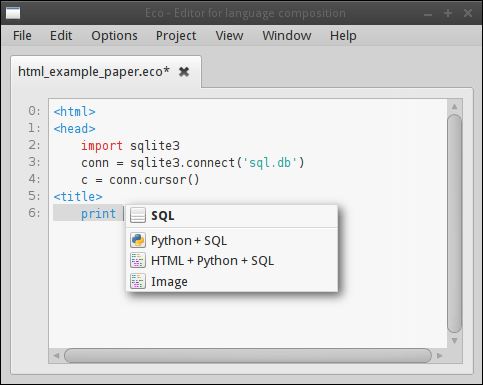
\includegraphics[width=0.5\textwidth]{images/dropdown.png}
\caption{Inserting a language box opens up a menu of the languages that \eco
knows about. Languages which \eco knows are valid in the current context are
highlighted in bold to help guide the user.}
\label{fig:langmenu}
\end{center}
\end{figure}

\begin{figure}[t]
\begin{center}
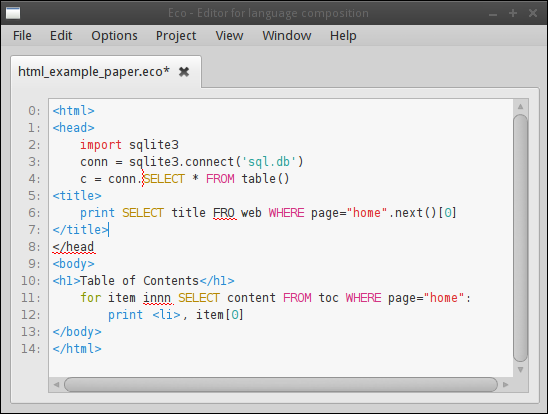
\includegraphics[width=0.5\textwidth]{images/errors.png}
\caption{Editing a file with multiple syntax errors.  Lines 6, 8 and 11
contain syntax errors in the traditional sense, and are indicated with
horizontal red squiggles. A different kind of syntax error has
occurred on line 4: the SQL language box is invalid in its current position
(indicated by a vertical squiggle).}
\label{fig:errors}
\end{center}
\end{figure}

Typing inside the Python+SQL language box makes it visibly grow on screen to
encompass its contents. Language boxes can be thought of
as being similar to the quoting mechanism in traditional text-based approaches
which use brackets such as $\llbracket~\rrbracket$; unlike text-based brackets,
language boxes can never conflict with the text contained within them. Users can
leave a language box by clicking outside it, using the cursor keys, or pressing
\hotkeyleavelbox. Within the parse tree, the
language box is represented by a token whose type is Python+SQL and whose
value is irrelevant to the incremental parser. As this may suggest, conceptually the top-level
language of the file (HTML in this case) is a language box itself. Each language
box has its own editor, which in this example means each has an incremental
parser.

At the end of the editing process, assuming that the user has a file with no syntax
errors, they will be left with a parse tree with multiple nested language boxes inside
it as in Figure \ref{fig:example1}. In other words, the user will have entered a
composed program with no restrictions on where language boxes can be placed; with no
requirement to pick a bracketing mechanism which may conflict with nested
languages; with no potential for ambiguity; and without sacrificing the ability
to edit arbitrary portions of text (even those which happen to span multiple
branches of a parse tree, or even those which span different language boxes).

\section{Using errors to detect language boxes}
\label{sec_finding_lbox_candidates}
% only on error
% glr style: check on every shift if a box is valid: subsection "Improving
% detection"

To humans it is often obvious where a user intended to embed a different
language.  For an algorithm however this is no easy task.  The challenge for
automatic language boxes is to find a heuristic that identifies as many
opportunities for the insertion of language boxes as possible. In order to not
interrupt the user, this heuristic must be fast.  More importantly though, we
must minimize the insertion of false positives, which would otherwise force the
user to perform unexpected manual work to revert the algorithm's mistakes which
is generally considered
unacceptable~\cite{vanter00displaying,lewis95designing,vanter94practical}.

A good indicator that a user may have wanted to insert a language box is when
the current program has a parsing error. Of course, not every error means a
language box was meant to be inserted, and not every language box the user
wants to insert is guaranteed to produce a parsing error. However, it is a good
initial heuristic, since languages often share similar keywords, or variable
names from one language may clash with keywords from the other.  This then
leads to parsing errors that can be fixed by surrounding the offending code
with a language box (see Figure \ref{fig_heuristic_example} for an example).

\begin{figure}
    \begin{subfigure}{0.4\textwidth}
    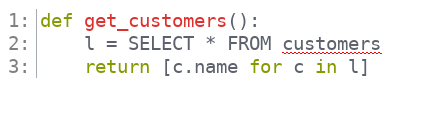
\includegraphics[width=1\textwidth]{images/heuristic1.png}
    \caption{Python and SQL}
  \end{subfigure}
  \begin{subfigure}{0.4\textwidth}
    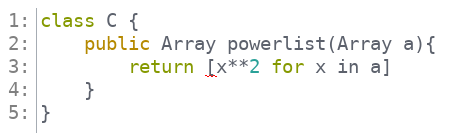
\includegraphics[width=1\textwidth]{images/heuristic2.png}
    \caption{Java and Python}
  \end{subfigure}
\caption{Two examples showing the attempted composition of languages without the
use of a language box. Both compositions result in an error, which can be used
to search the surrounding for potential language box locations. \textbf{a)}
Here we have to search backwards to \texttt{SELECT} at which location the
insertion of an SQL box is possible. \textbf{b)} Here a box can be inserted
immediately at the location of the error.}
\label{fig_heuristic_example}
\end{figure}

To decide if a parsing error can be fixed via insertion of a language box, we
need to analyse errors as soon as they appear during the parsing process. This
has the advantage that we have additional parsing information available, like
the parse stack, to help us decide whether the insertion of a box is a valid
and sensible choice. Analysis of the errors is done by the new automatic
language box detector, which we will call \ald from here on. The basic idea is
that when an error is encountered, we search for language box candidates whose
insertion around the error would render the input successful. The main
challenge is therefore in finding suitable candidates.

We start by searching backwards from the error to find locations where a
language box would be valid. From here, for each language in the composition,
we then try to match as much text as possible. If consumed text is valid in one
of the languages, a candidate is produced. Each language can produce multiple
candidates by consuming more text, even if a candidate for that language has
already been produced. Afterwards, each candidate language box is virtually
applied to the user's input (replacing the consumed text). If it introduces
extra errors or does not fix the initial parsing error, the candidate is
discarded. The algorithm for finding candidates is shown in Listing
\ref{lst_find_candidates}.  If at the end no candidates are found, the error
remains, as normal; if one candidate is found, we automatically insert the
appropriate language box; and if multiple candidates are found, we ask the user
for help.

\begin{figure}[t]
\begin{lstdefault}
def find_candidates(error):
  valid_boxes = []
  for lang in <!\textit{composition}!>:
    cut = len(stack)
    while cut >= 0:
      if <!\textit{lbox of lang can be shifted at cut}!>:
        valid_boxes.append((lang, cut))
      cut -= 1

  candidates = []
  for lang, cut in valid_boxes:
    results = consume_text(stack[cut], lang)
    for r in results:
      candidates.append((lang, cut, r))

  f = []
  for c in candidates:
    if confirm_candidate(c) and fixes_error(c, error):
      f.append(c)
  return f
\end{lstdefault}
\caption{Algorithm for finding language box candidates, for readability divided into
several steps. First, for each language $l$ in the composition, we scan the text
before the error to find valid locations where a language box of $l$ can be
inserted -- this step is similar to and was inspired by the finding of isolation
nodes, in that it also uses the parse stack to find such locations (lines 2--8). For each of
those locations we then try to consume its following text, using $l$'s lexer and
parser, and produce a candidate whenever the consumed text is a valid program in
$l$ (lines 10--14); \texttt{consume\_text} stops when we can't consume any more text, because either the remaining
text is invalid in $l$, or there is no more text to consume. Afterwards, we
confirm the produced candidates by checking if they fix the previous error and
don't introduce any new ones (lines 16--19).
Candidates are returned in the order they are found: the closer to the error and
shorter they are, the higher they are in the list.}
\label{lst_find_candidates}
\end{figure}

Even though language box candidates are found during parsing, they are only
inserted (either automatically or via selection by the user) after parsing has
finished. The reason for this is simply that inserting them after parsing
triggers another reparse, which then creates a new parse tree version. This
allows us to easily undo automatically inserted language boxes again by simply
going back to the parse tree version just before the language box was inserted.
To undo an automatic insertion, the user simply needs to press \keys{Ctrl+Z}.
When the user reverts an automatic language box insertion, the editor remembers
this decision and does not attempt to insert the same language box again, so
that the user doesn't have to repeatedly fix the algorithm's mistakes.

\subsection{Finding candidates}

As an example, let's consider a composition of Java and Python, where Python
functions are allowed wherever Java functions are valid. For this we embed into
Java a subset of the Python grammar, accepting only Python functions, which we
call \texttt{pyfuncdef}\footnote{This grammar can be constructed from the
Python grammar (shown in Appendix \ref{app_python_grm}) by changing the start
rule to \texttt{funcdef}.}. We now assume the user wrote the following program:

% Normal example
\begin{lstdefault}[language=Java]
  class Example {
      def x():
  }
\end{lstdefault}
\vspace{1em}

This program currently has a parsing error at \qtt{:}\footnote{The parser
expected an opening bracket here, as Java parses \qtt{def x()} as a function
definition \qtt{x} of the type \qtt{def} which needs to be followed by opening
and closing brackets.}. We now try to find a valid location on the parse stack,
where a \texttt{pyfuncdef} language box can be pushed, which we find just
before \qtt{def}.
In the next step we try to find candidates by consuming text, starting at
\qtt{def}.  The language \texttt{pyfuncdef} can consume everything up to, but
excluding \qtt{\}}, which causes a parse error and thus cannot be consumed. The
only consumed text up to that point is \qtt{def x():}, which is not a valid
program in \texttt{pyfuncdef}, and so no candidate is produced as a result.

Assume now that the user inserts \qtt{pass} into the above program, resulting in:

\begin{minipage}{\linewidth}
\begin{lstdefault}[language=Java]
  class Example {
      def x():
          pass
  }
\end{lstdefault}
\end{minipage}
\vspace{1em}

While the error remains at \qtt{:}, more text can be consumed this time. Again,
we use the language \texttt{pyfuncdef} to consume text starting from \qtt{def}.
Upon consuming \qtt{pass}, a valid Python function has been found and a
candidate is created. We continue consuming text, to find further candidates.
However, as before, we stop upon reaching \qtt{\}} which is not valid in
\texttt{pyfuncdef}. Having found a candidate, we now need to check if it fixes
the error and doesn't introduce any other errors immediately following the box,
when it's applied to the users input. We replace the consumed text with a
language box of \texttt{pyfuncdef} and start a reparse in the outer language,
Java, at its location. As soon as we successfully parsed \qtt{\}} we can stop
the reparse, confirming that the insertion of the candidate doesn't introduce
any new errors (Section \ref{sec:parse_after_lbox} discusses why it is
sufficient to stop parsing after \qtt{\}} and why we don't have to parse the
entire program to determine if the candidate is valid).  Finally, we check if
the original error has been eliminated, which is the case here, as the error
node \qtt{:} was included in the candidate language box. The candidate is thus
a valid candidate and can be automatically inserted into the program.

\subsection{Confirming candidates}
\label{sec:parse_after_lbox}

In order to confirm if an automatic language box candidate is valid, we need to
check that it does not introduce new errors when it is inserted into the parse
tree, and also that is fixes the initial parsing error.  To check if a
candidate doesn't introduce new errors, we can simply check if the first
non-whitespace token that follows it can be shifted.  The reasons for this are
twofold. Firstly, we don't want to parse too far past the language box, for
performance reasons, and because this could lead to candidates being falsely
rejected (see Figure \ref{fig_autoboxerrorafterinsert} for an example).
Secondly, whitespace tokens, which most programming languages use, have the
property, that they can almost always be shifted after another terminal. This
means that a whitespace token following a language box candidate would always
confirm the candidate, even if the insertion of the box would cause an error
immediately after that whitespace. This can sometimes lead to invalid
candidates being accepted (see Figure \ref{fig_autobox_nonwhitespace} for an
example).

\begin{figure}
\begin{center}
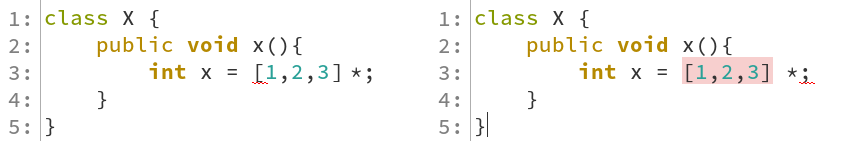
\includegraphics[width=0.50\textwidth]{images/autoboxerrorafterinsert.png}
\end{center}
\caption{An example showing why parsing further than necessary to confirm
a language box candidate, can lead to the candidate being falsely rejected.
The example shows a composition of Java and Python, that allows Python
expressions wherever Java expressions are valid. The user inserted a Python list
into the program (left), which produced a language box candidate (right). To validate
the candidate we insert it into the program and parse it. However, after parsing \qtt{*},
an error occurs which would invalidate the constraint that an automatic
language box shall not introduce new errors, and thus reject the candidate,
despite this being an otherwise valid insertion.}
\label{fig_autoboxerrorafterinsert}
\end{figure}

\begin{figure}
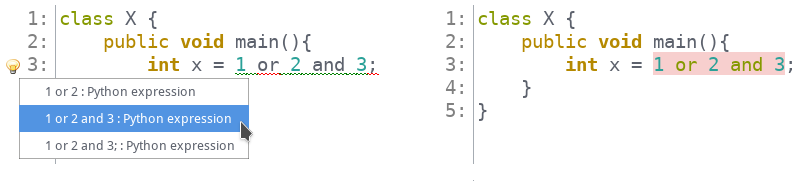
\includegraphics[width=0.5\textwidth]{images/autobox_nonwhitespace.png}
\vspace{0.3em}
\caption{An example showing how using only non-whitespace tokens to confirm language
box candidates gives better results. The example uses a composition of Java
and Python, which allows Python expressions in place of Java expressions. The
user just pasted the Python code \qtt{1 or 2 and 3} into the assignment, in
between \qtt{=} and \qtt{;}. \textbf{a)} If we use any first token to confirm
candidates, we get three results. The first option, \qtt{1 or 2},
is a valid candidate, because the following token is whitespace, which can
be shifted, confirming the candidate; however the following
\qtt{and} then causes an error. The same is true for the third option, \qtt{1 or 2 and 3;}, which is
followed by a newline, which confirms this candidate, even though the \qtt{\}} then
errors because the semicolon of the assignment was included in the Python
language box. \textbf{b)} When using the first non-whitespace token for candidate
confirmation, we reduce the three options to one, which can then be automatically
inserted.}
\begin{picture}(0,0)
  \small
  \put(-110,225){\textbf{(a)} Using first token}
  \put(-20,225){\textbf{(b)} Using first non-whitespace token}
\end{picture}
\label{fig_autobox_nonwhitespace}
\end{figure}

% Multiple choice example
\subsection{Handling multiple solutions per language}

While many compositions only have one valid outcome, sometimes there are
multiple options for the insertion of a language box. This can be either that
there are multiple languages that can be inserted, or that there are multiple
variants of consumed text for a single language.  An example for the latter is
shown in the following composition of PHP and Python, which allows any Python
box wherever a PHP expression would be valid.

\begin{center}
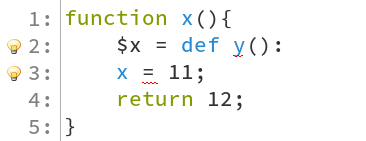
\includegraphics[width=0.25\textwidth]{images/autoboxmultioption.png}
\end{center}

In the example there are two options to fix the error at \qtt{y} in line 2, via
the insertion of a Python box. We can include everything from \qtt{def} up to,
and including \qtt{return 12}, or we can stop after \qtt{x = 11}.  Since both
options are valid and fix the error, we can't automatically pick one.
Instead, we display an indicator that there are multiple solutions available
(in \eco this is done via a light bulb icon next to the line numbers). From
there the user can choose one of the solutions from a drop-down list. Clicking
on one of the options then automatically inserts a language box and replaces
the relevant code:

\begin{center}
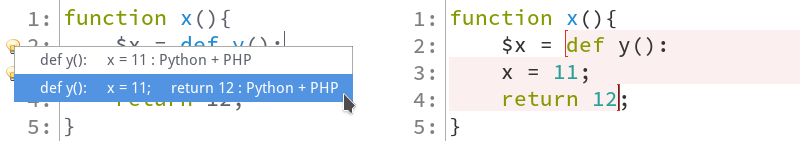
\includegraphics[width=0.50\textwidth]{images/autoboxmultioption2.png}
\end{center}

\subsection{Limiting automatic insertions}
\label{subsec:limitingautoinserts}

Some grammars can be very unrestrictive, allowing almost any text to be valid.
In HTML, for example, any combination of characters that does not contain
\qtt{<} or \qtt{>} is a valid program. Unfortunately, this means that in a
composition with HTML most errors can be solved by simply wrapping them with a
HTML language box, often resulting in something the user didn't intend. For
instance, the following example shows a program written in a composition of
Python that allows SQL and HTML wherever Python expressions are valid:

\begin{center}
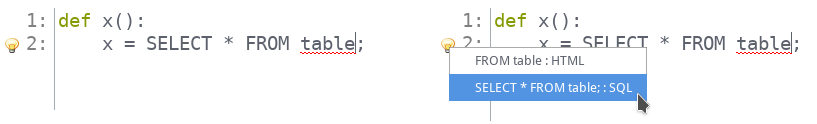
\includegraphics[width=0.5\textwidth]{images/auto_html.png}
\end{center}

We can see that the error at \qtt{table} can be solved by either wrapping
\qtt{SELECT * FROM table} into a SQL language box, or by just wrapping
\qtt{FROM table} into a HTML language box. To a human, however, it is obvious
that the user meant to insert a SQL box here. While this is impossible for the
algorithm to detect, the creator of the language composition can add hints that
limit the insertion of some language boxes in certain scenarios.  For example,
for the above, we could define that a HTML box should only be inserted if the
box starts with a HTML tag, e.g.~\qtt{<img}.  When composing languages, \eco's
language composition interface provides a function \texttt{add\_limit(lang,
tokens)}, which takes as input the sublanguage we want to limit, and a list of
tokens which are allowed to trigger automatic language box insertion.  This way
we can restrict the Python and HTML composition and solve the above problem,
via the simple addition of \texttt{pythonhtml.add\_limit("HTML",
["tag\_open"])}.

Of course, another valid solution would also be to simply define a more
fine-grained composition. For example, instead of creating a Python/HTML
composition that allows all HTML to be valid wherever Python expressions are
valid, the composition could be restricted to only allow HTML-tags
(e.g.~\qtt{<img}, \qtt{<html}, etc) by embedding only a subset of the HTML
grammar.  Although, this may not always be possible if the grammar doesn't
separate rules on such a fine grained level.

\subsection{Automatically removing boxes}
\label{subsec_autoremoval}

Despite the solutions described in \ref{subsec:limitingautoinserts} it is
impossible to always predict where language boxes should be inserted and there
will be cases where automatically inserted language boxes do not match the
user's intentions. While the user can always undo a wrong insertion by pressing
\keys{Ctrl+Z}, we do not want to burden them with the task of repeatedly
cleaning up the algorithm's mistakes.  The following composition of Python and
SQL, though admittedly a rather unlikely scenario, exemplifies the problem:

\begin{lstdefault}[language=Python]
  def x():
    SELECT = 1
    FROM = 2
    table = 3
    x = SELECT * FROM table
\end{lstdefault}
\vspace{1em}

After typing in this program, an SQL language box will have been automatically
inserted, replacing the text \qtt{SELECT * FROM table}. From a syntax
perspective, this was a valid decision. However, we can see from the variable
declarations that the user's intention was to multiply the three poorly named
variables and simply forgot a \qtt{*} between \qtt{FROM} and \qtt{table}.
Instead of requiring the user to manually undo the insertion, \eco can
automatically remove inserted language boxes again once more information has
become available.  In this example, once the user inserts the missing \qtt{*}
between \qtt{FROM} and \qtt{table}, the SQL language box becomes invalid. This
gives us a good clue that the language box was inserted accidentally and needs
to be removed; with the restriction, that its entire content can be parsed in
the outer language.
However, sometimes an automatically inserted language box can become valid in
both the inner as well as the outer language, after the user made additional
changes.  In those cases \eco prioritises the outer language and removes the
box, but only if the boxes contents \emph{and} its surrounding context can be
parsed in the outer language.  The following constraints summarise the above
(an example using the constraints is given in Figure \ref{fig_autoremoval}):
\begin{enumerate}
  \item Only automatically inserted boxes can be automatically removed again.
  \item If the language box content is invalid, it will be removed only if
        its content can be parsed in the outer language.
  \item If the language box's content is valid in both the inner and outer
    language, it will be removed only if its removal doesn't introduce new errors (i.e.~if its contents \emph{and} the first non-whitespace token following it
    can be parsed).
\end{enumerate}

Using these constraints for the example from before, the inserted box would be
removed as soon as the user inserts a \qtt{*} between \qtt{FROM} and
\qtt{table}; however, it stays if more SQL code is added even it that makes the
SQL box temporarily invalid. Note that language boxes that were inserted by the
user, via choosing one of the suggested candidates, count as manual insertions
and won't be automatically removed, even if they become invalid.


\begin{figure}
\begin{center}
\vspace{0.8em}
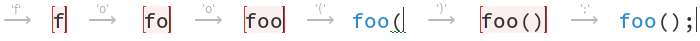
\includegraphics[width=0.45\textwidth]{images/autoremove_foo.png}
\vspace{-0.8em}
\end{center}
\caption{An example showing the constraints for automatic language box removal in practice.
The example uses a composition of PHP and Python where Python expressions are valid at
PHP's top-level.
We can see that as the user types, language boxes are getting automatically
inserted and removed depending on their content. At the beginning the user types
\qtt{f}, which is not valid in PHP and thus gets replaced by a Python
language box, making the program valid again. The box stays until the user
inserts \qtt{(} which makes the Python language box invalid, and since all of
its content can be parsed in the outer language, the box is removed.
As soon as the user inserts the closing bracket \qtt{)}, a Python box is
inserted again to fix the PHP parsing error caused by a missing semicolon. When the
user eventually inserts the missing semicolon the contents of the language box
are valid in both PHP and Python. However, since the box can be removed
without introducing an error, we prioritise the outer
language, and remove it again.}
\label{fig_autoremoval}
\end{figure}

%After a language box has been inserted it stays in a "to be determined"
%mode. When the user moves the cursor outside the box, the box is finalised. Until then,
%any changes inside the box have to be validated and can lead to the box being destroyed again.
%E.g. changing \qtt{x = SELECT * FROM table;} to \qtt{x = SELECT * FROM} will remove the box again
%as the content is valid Python now and not valid SQL anymore.


\section{Limitations}
\label{sec_lbox_limitations}

This section gives some examples of ambiguities that cannot be resolved with
automatic language boxes and thus display their limitations. This results in
unwanted language boxes being inserted, or no language boxes being inserted,
opposing the user's intentions.

\subsection{No detection}

One example, where error based detection of automatic language boxes doesn't
work, is when the outer language can match everything in the inner language.
For example, HTML can match arbitrary text between tags. This makes
compositions, where other languages are embedded into HTML, impossible to
detect automatically. The following code example shows this:

\begin{lstdefault}[language=html]
<html>
import sqlite
sqlite.connect("test.db")
</html>
\end{lstdefault}
\vspace{1em}

Since HTML allows any text in between its tags, the insertion does not cause an
error, and thus the \ald is never called to detect automatic language boxes.
However, even to a human it is unclear if the user meant to insert a Python
box, or simply wanted to print out the code in HTML. Although, a non-error
based heuristic for finding language box candidates could at least show the
user that a language box would be possible.  A naive example for such a
heuristic could try to match language boxes at each terminal location. However,
such a solution would be much slower than the error based approach.

\subsection{Wrong detection}

Another problem is when the insertion of an automatic language box extends into
parts of the outer language, even if those parts weren't meant to be included
inside of the box. For example, this can occur when composing Java and Python,
allowing Java functions to be replaced with Python functions, as shown below:

\begin{center}
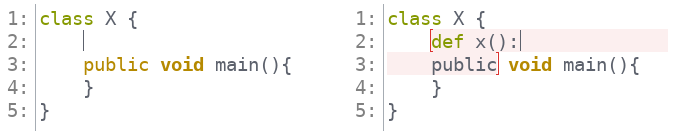
\includegraphics[width=0.50\textwidth]{images/autobox_limitjavapy.png}
\end{center}

The user attempted to insert a Python function above the Java function.
However, as the user was typing, a box was automatically inserted which
extended into the Java function, and used the keyword \qtt{public} as the body
of the Python function.  This is valid, since the keyword is optional in Java,
so the insertion of that box does not create any errors, even though it is
clearly not what the user intended.

\subsection{Grammar limitations}

Sometimes the structure of a grammar can be responsible for the failure to
generate automatic language boxes. For example, let's consider a composition of
PHP and Python, that allows Python expressions wherever PHP expressions are
valid, into which the user types the following input:

\begin{center}
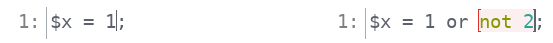
\includegraphics[width=0.45\textwidth]{images/autobox_limitphpgrammar.png}
\end{center}

The user might reasonably expect to have a second option here, which would
allow the content \qtt{1 or not 2} to be wrapped into a Python language box.
The algorithm, however, couldn't detect this and instead only found a single
candidate, \qtt{not 2}, which was automatically inserted.  The problem lies
within the PHP grammar, which also has a keyword \qtt{or}, and how the location
for language box candidates are calculated. As described earlier in this
chapter, we use a technique similar to error recovery, that rewinds the parse
stack to find a position on the stack, where the language can be inserted.
However, the way the PHP grammar is structured and thus parses the above input,
makes it impossible to find a location on the stack that allows \qtt{1 or not
2} to be wrapped into a language box, as Figure \ref{fig_auto_phplimit} shows.

\begin{figure}
\begin{center}
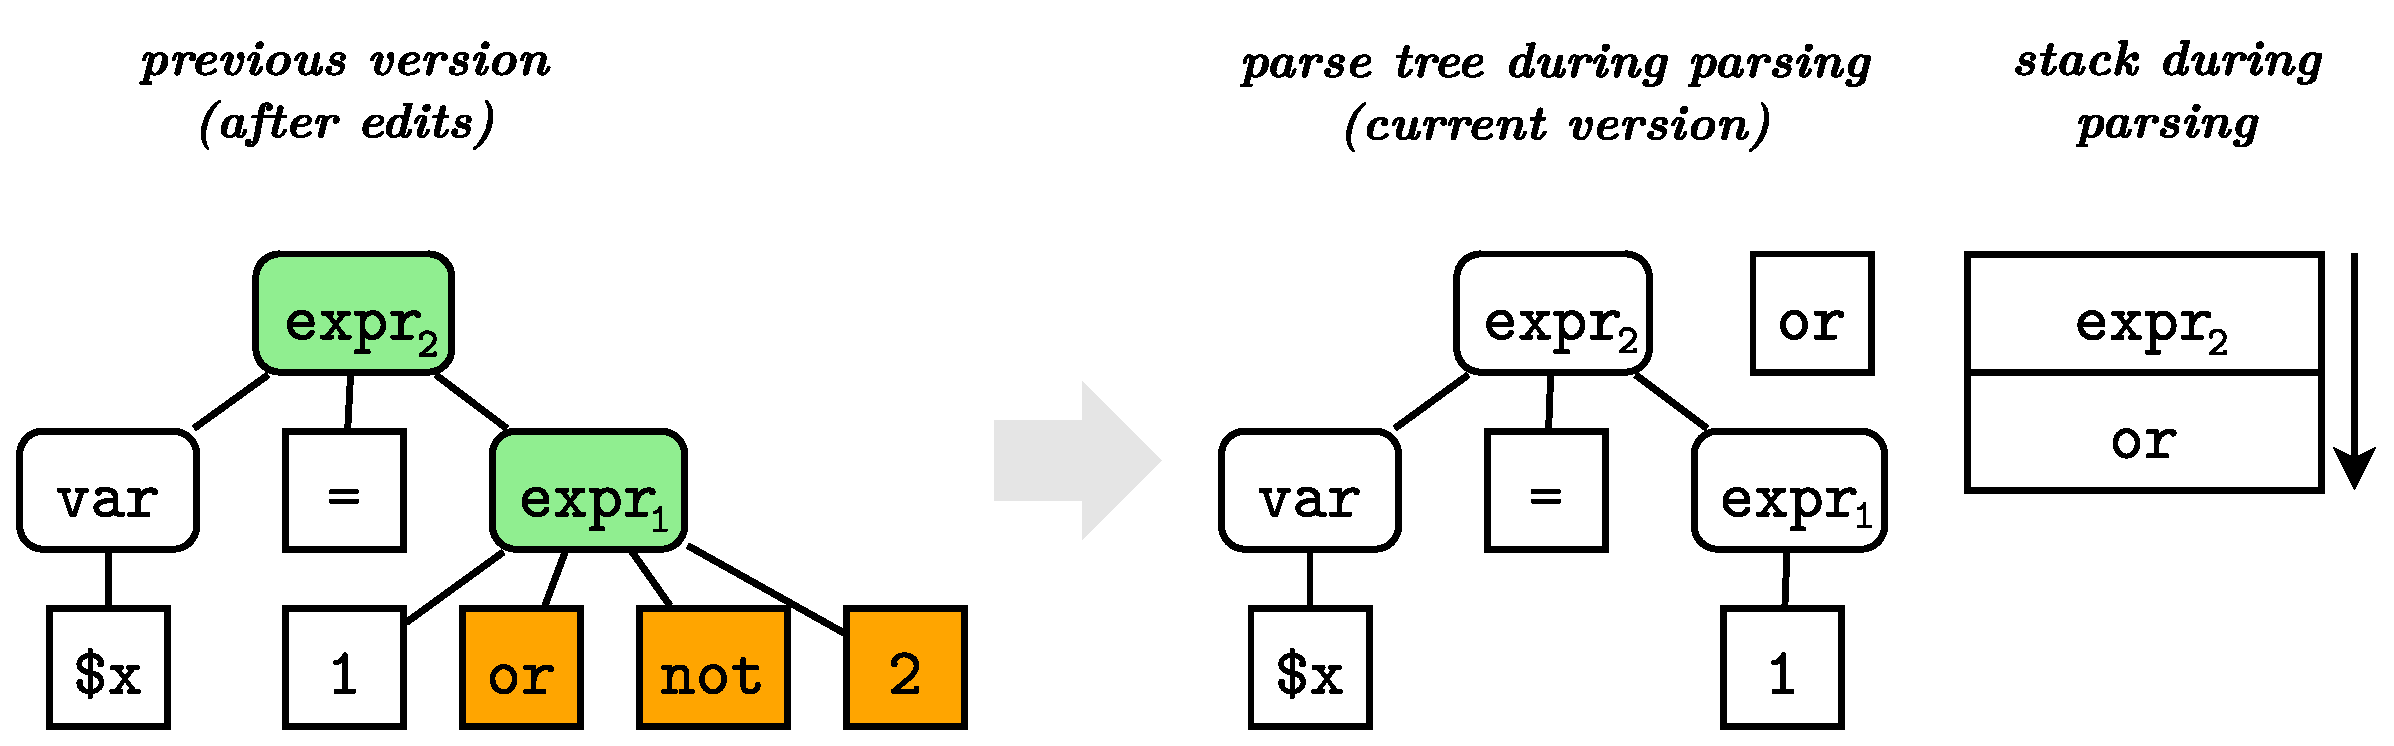
\includegraphics[width=0.49\textwidth]{images/limitation_php}
\end{center}
\caption{An example showing how sometimes the grammar of a language can
keep the automatic language box detection from finding appropriate candidates.
On the left is shown the elided parse tree after the user edited the PHP expression
\qtt{\$x = 1;} by inserting the Python code \qtt{or not 2}. However, we
can see on the right, that by the time the error occurs, PHP has already reduced \qtt{\$x = 1} to \texttt{expr\textsubscript{2}}, and shifted
\texttt{or} onto the stack. The only valid locations for a language
box we can thus find are before \texttt{expr\textsubscript{2}} and \texttt{or}. In particular,
we cannot find the location before \qtt{1} which would allow us to wrap the entire expression
into a box.}
\label{fig_auto_phplimit}
\end{figure}

\section{Recognisers}
\label{sec:impl_defaultrec}

This section describes in more detail how language box candidates are
constructed and how we can improve performance by not using a full incremental
parser to find language box candidates, but instead using a simple batch
recogniser. A recogniser is a parser that doesn't execute any actions or
generates a parse tree, but rather only validates the input. This section also
shows how a recogniser can be used to decide whether or not a language box can
be removed again.

Section \ref{sec_finding_lbox_candidates} described, how in order to find
language box candidates, we try to consume as much text surrounding the error
node as possible, generating a candidate every time the surrounding text is
valid in the language of the box. Since we are only interested in the text that
can be parsed and don't need to generate a parse tree from it, a simple batch
recogniser is a good alternative to a full parser, as it improves performance
and reduces memory usage.  An important restriction is that the recogniser must
lex and parse input from the parse tree without actually altering the parse
tree or any nodes within it.  A recogniser in the \ald takes as input a node
from which it starts parsing, and returns all valid substrings from that input,
until either a parsing error occurs, or there is no more input left to parse.
Substrings are returned in form of their end node in the original parse tree.
The substring can then be derived by reading all tokens between the start and
end node.  The algorithm is shown in Listing \ref{lst_consume_text}.

\begin{figure}
\begin{lstdefault}[]
def consume_text(node, lang):
  lexer = <!\textit{lexer for lang starting at node}!>
  parser = <!\textit{parser for lang}!>
  results = []
  token = lexer.next_token()
  while token is not None:
    if parser.parse(token):
      if <!\textit{parser can accept current input}!>:
        results.append(lexer.last_node)
    else: # parse error
      break
    token = lexer.next_token()
  return results
\end{lstdefault}
\caption{An algorithm for consuming text and returning valid
substrings for the creation of language candidates. We first create a lexer that
produces tokens in language \texttt{lang}, starting at \texttt{node} (line 2).
We also create a parser for \texttt{lang} (line 3) which is used to parse input (line 7) and test if the
input parsed so far can be accepted (line 8); the latter can be achieved by simply pretending
that the next token is the end-of-file token, and test if the
parser reaches an accept state. We then consume as much text as we can,
producing tokens and parsing them (line 6--12), until no more text can be
consumed, either due to an error (line 10), or because we've reached the end of
the input. Each time a token was successfully parsed, we test if the input parsed so far is
valid (line 8), and if so, store the last node from the original parse tree that the lexer
processed (line 9). This node is later used to derive the substring from which the
language box is created.}
\label{lst_consume_text}
\end{figure}

\subsection{Custom recogniser for Python}
\label{sec:impl_wsrec}

In order to produce language box candidates for whitespace-sensitive languages
like Python, we need to be able to create indentation tokens during the
consumption of input. Section \ref{sec:indentation} described how support for
whitespace-sensitive languages was added by allowing an additional phase
between lexing and parsing that inserts indentation tokens into the parse tree.
This method can't be used here, since we do not know yet where the input ends.
Fortunately, since the recogniser is not incremental (and doesn't need to be),
this is not necessary and indentation tokens can be generated on the fly. To do
this, the recogniser for Python uses a wrapper around the lexer which inspects
the tokens that the lexer produces and, when appropriate, returns indentation
tokens instead. While the Python recogniser inherits most of the behaviour of
the default one, it also needs to keep track of the indentation levels. Listing
\ref{lst_next_token_indent} shows how the recogniser wraps around the lexer and
produces indentation tokens whenever they are needed.

\begin{figure}
\begin{lstdefault}[basicstyle=\linespread{1.0}\footnotesize\ttfamily]
def next_token(todo, indent):
  if todo:
    return todo.pop(0) # return first element
  token = lex.next_token()
  if token is <!\textit{newline}!>:
    prevl = <!\textit{previous line}!>
    currl = <!\textit{current line}!>
    if prevl is not empty:
      todo.append(<!\textit{NEWLINE}!>)
    if currl is not empty:
      if prevl.ws < currl.ws:
        indent.append(currl.ws)
        todo.append(<!\textit{INDENT}!>)
      elif prevl.ws > currl.ws:
        ws = indent.pop()
        while ws > currl.ws:
          todo.append(<!\textit{DEDENT}!>)
          ws = indent.pop()
        if ws != currl.ws:
          todo.append(<!\textit{UNBALANCED}!>)
  todo.append(token)
  return todo.pop(0)
\end{lstdefault}
\caption{To support language box detection for Python, we
create a method that wraps around the lexer and produces indentation tokens as
needed by keeping track of the indentation levels. Producing and returning
indentation tokens delays the parsing of tokens which have already been lexed.
In order to not forget to parse those tokens, we use a to-do list (line 3). We
always return the first item of that list. If it is empty, we continue lexing
from the input (line 4). The remaining code is similar to the batch indentation
approach described in Section \ref{subsec_indentation_batch}.
}
\label{lst_next_token_indent}
\end{figure}

\subsection{Incremental Recogniser for auto removal}
\label{sec:impl_removerec}

Section \ref{subsec_autoremoval} described how automatically inserted language
boxes can automatically be removed again, if they become invalid. The condition
for this is that the box's content is valid in the outer language.  In essence,
we need to temporarily remove the language box, paste its content where the box
was before, and then check if the program can still be parsed; of course
without actually altering the parse tree. A recogniser is thus again a good
choice. In order to test if the contents of the box are valid in the outer
language, we first need to initialise the recogniser to the state just before
the language box would be parsed. We can do this incrementally, by only
traversing subtrees that are direct ancestors of the language box. All other
subtrees can be skipped (i.e.~incrementally shifted) similar to the default
incremental parser.

This process is implemented via an additional method \texttt{preparse}, which
incrementally initialises a recogniser's parsing state to the state just before
a given node. Figure \ref{fig_preparse} shows an example of a parse tree, where
we want to test if a language box can be removed, and the algorithm to
initialise the recogniser.
After the recogniser has been initialised, we simply use \texttt{consume\_text}
to parse the content of the language box. If the entirety of the language box
can be successfully parsed in the outer language, the box can be removed.  Of
course, depending on the parsing status of the box, we may also need to parse
at least one non-whitespace token following the former language box.

\begin{figure}
\begin{minipage}{0.45\textwidth}
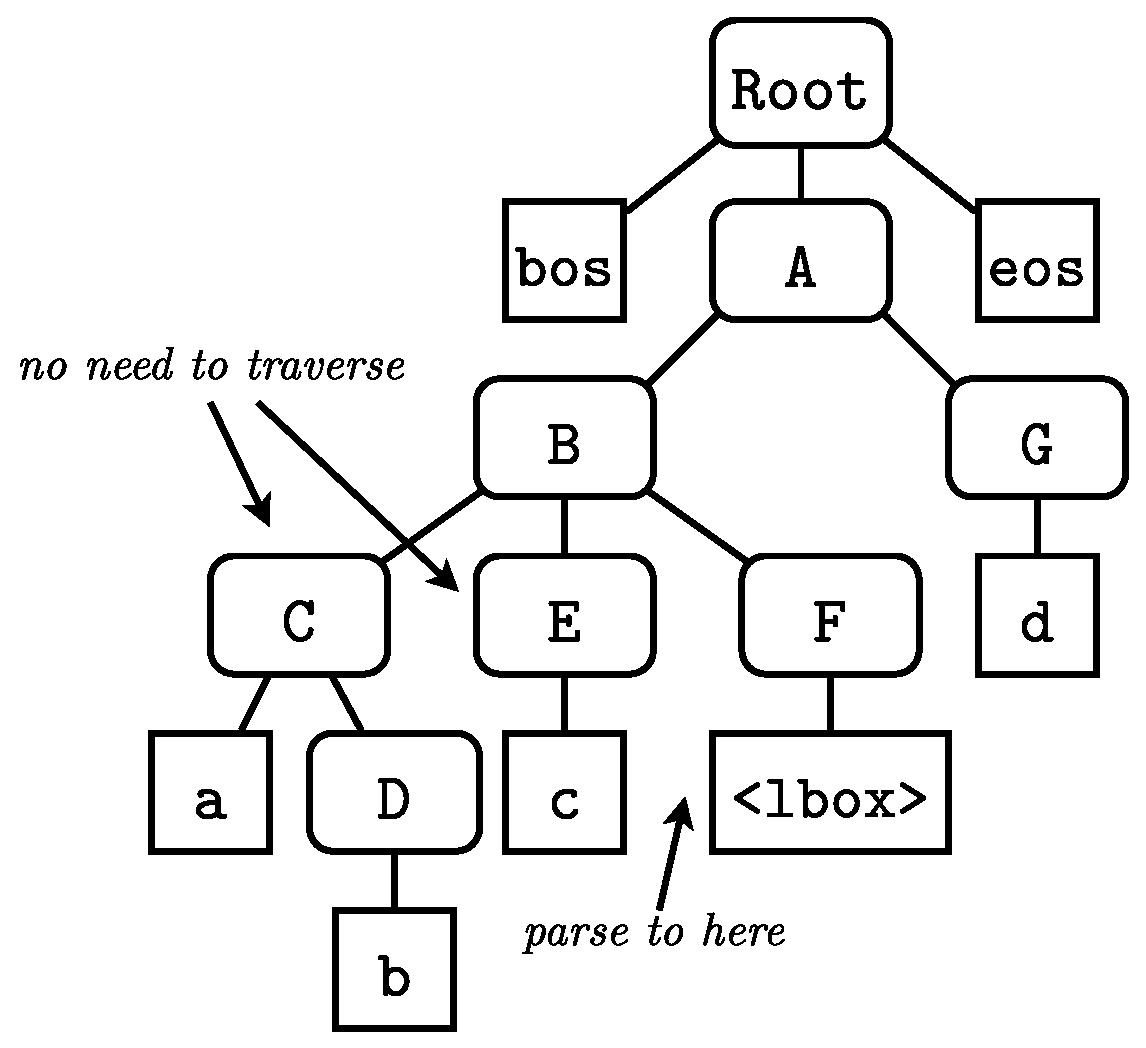
\includegraphics[width=0.9\textwidth]{images/autoremoval}
\end{minipage}
\begin{minipage}{0.5\textwidth}
\begin{lstdefault}[basicstyle=\linespread{1.0}\footnotesize\ttfamily]
def preparse(bos, lbox, parser):
  # "mark" ancestors of lbox
  path_to_lbox = set()
  parent = lbox.parent
  while parent is not <!\textit{Root}!>:
    path_to_lbox.add(parent)
    parent = parent.parent

  # initialise parser
  node = bos
  while node is not lbox:
    if node not in path_to_lbox:
      parser.parse(node)
    else: # traverse node
      if node.children:
        node = node.children[0]
      else:
        node = node.right_neighbour()
\end{lstdefault}
\end{minipage}
\caption{A parse tree with a language box that we want to automatically remove (left)
and the preparse-algorithm (right). In
order to test if the box's content is valid in the outer language, we
initialise a recogniser to the state just before we would parse the language box,
using the recogniser's \texttt{preparse} method. This is done,
by `marking' the ancestors of the language box, as if the language box
contained changes (lines 3--7), and then incrementally parse those subtrees
up to the box (lines 10--18).}
\label{fig_preparse}
\end{figure}

\section{Related Work}
\label{autobox_related_work}

The following discusses two other examples for language composition that are
related to language boxes.

Scannerless parsing~\cite{visser97scannerless, vandenbrand02disambiguation} is well
suited for language composition since it can parse any context-free grammars
which are closed under composition. A notable example of this is
Spoofax~\cite{kats10spoofax}, a language workbench for extending and composing
context-free grammars. However, Spoofax's grammar definition SDF, which allows
arbitrary CFGs, can give no guarantees that its grammars are unambiguous, even
more so when they are composed together, since composing two unambiguous
grammars can lead to an ambiguous one.  Spoofax thus uses reject grammars,
which solve this problem, but make such grammars
context-sensitive~\cite{eijck__lets_accept_rejects}.

Another notable example for language composition is Copper~\cite{wyk07context}
which implements a context-aware scanner to solve ambiguities in language
compositions. The basic idea is that the parser can tell the scanner which
tokens it can parse next and the scanner can only return results from that
list.  This means that if two composed languages have similar tokens
(e.g.~keywords, identifiers), the lexer solves ambiguities by returning the
token for the language that it is currently parsing (i.e.~that is currently in
context). This allows Copper to compose languages by extending the host
language's grammar rules with references to rules in the embedded language.
However, at the point where another language can be embedded, i.e.~where the
two languages meet, a token may be valid in both the host as well as the
embedded language.  Copper solves this problem via \texttt{dominates} clauses
which are defined within the lexing rules. For example, if an identifier in the
host language clashes with a keyword in the embedded language, then we can
define a clause that says that the keyword dominates the identifier and needs
to be prioritised. Unfortunately, this has the downside that those tokens
cannot be used in the host language at that point, restricting the host
language's expressiveness. This also means that each composition needs to
determine all of those cases and modify grammar and lexer in ways that solve
these ambiguities, making it impossible to create a one-size-fits-all solution
for arbitrary compositions.

\bibliography{bib}

\end{document}
